\subsubsection{Product Browser}
The Product Browser was implemented as follows:
\begin{description}
\item[Product Search] This was implemented as ProductSearch, a PopupPanel which allows the user to 
search for products by name, as well as by category and/or location. This then sends the search request
 to the Datastore via WebPage, WebSystem and RPC and directs the user to
 ProductList.
 \item[Product Viewer]This was implemented as ProductList, which presents the
 user with a tabular display of the products they searched for. It contains buttons to access ProductDetail and GraphTypePopup.
\item[Info Popup] This was implemented as ProductDetail, a popup which displays
extra information about a chosen product.
\item[Graph Chooser] This was implemented as GraphTypePopup, a PopupPanel
which allows the user choose what type of chart they which to view, in terms of
which products they wish to have displayed. This will then take the user to
the Graph Viewer.
\end{description} 
\begin{figure}[h!]
\centering
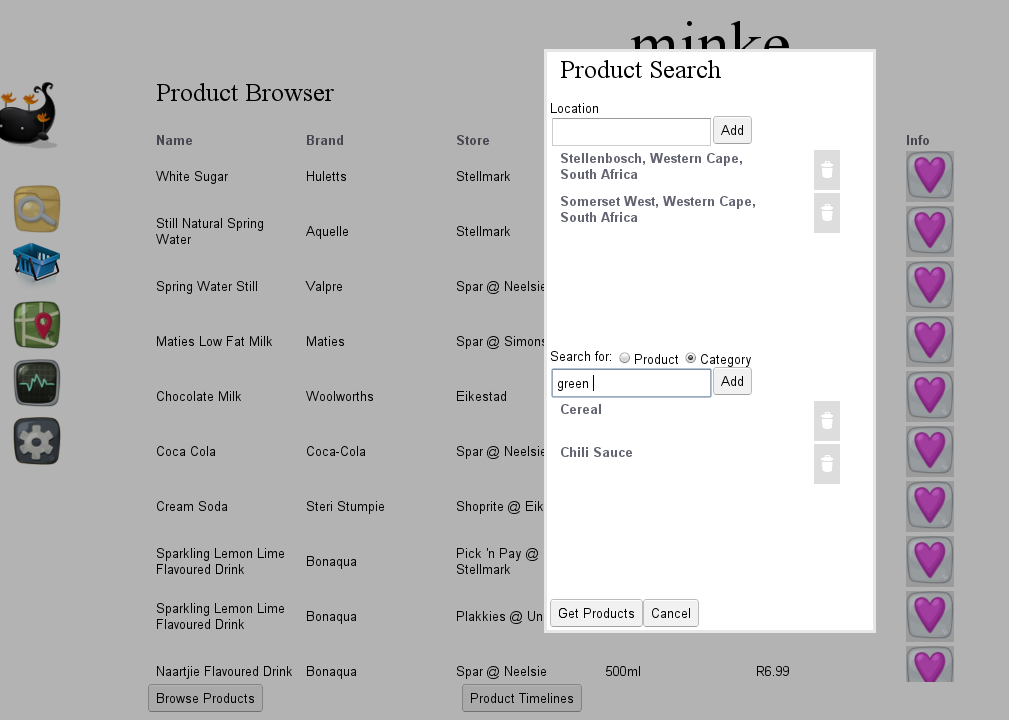
\includegraphics[width=0.8\textwidth]{gwt-search.png}
\caption{Product search interface with viewer in background.}
\end{figure}